% ============================ RESEARCH PAPER ==================================
\phase{Phase eight \textbullet\ The paper}{Do India's green-ammonia auctions clear below cost?}{The research design, the first results on all 65 bids, the literature it builds on, and what still has to be done before submission.}\label{sec:paper}

\subsection{The question}
In 2025, SECI ran thirteen e-reverse auctions under SIGHT Mode 2A to buy 724,000 tonnes a year of green ammonia for Indian fertiliser plants, on ten-year contracts \cite{seci2025}. The volume-weighted winning price was \textbf{₹53.27/kg}. Dossier 1 found that the winning bids quietly assume a hydrogen cost of about \usd{}2.5--2.9/kg, well below what a typical developer can deliver today. That suggests a sharp, testable question:

\begin{center}
\begin{minipage}{0.9\textwidth}\centering
\display\itshape\fontsize{12.5}{16}\selectfont\color{ink}
Do India's green-ammonia auctions clear below the probabilistic cost of delivery? A stochastic levelised-cost and real-options assessment of winner's-curse risk in SECI's SIGHT Mode 2A.
\end{minipage}
\end{center}

\noindent The \emph{winner's curse} is the old observation that in a competitive auction for something of uncertain cost or value, the winner tends to be the bidder who was most optimistic, and so is systematically likely to have got it wrong \cite{capen1971,thaler1988}. If it is happening here, the policy consequence is serious: contracts that are awarded but never delivered, as has happened to under-priced renewable auctions before. We are not aware of a published study that tests these auctions for it. \confM

\subsection{Three hypotheses, three tests}
\begin{center}\tablefont
\begin{tabularx}{\textwidth}{@{}P{8mm} L L@{}}
\toprule
\thead{} & \thead{Hypothesis} & \thead{Test}\\ \midrule
H1 & Bids are bunched more tightly than cost differences between bidders would justify. & \textbf{Bid structure:} gap between winner and runner-up; dispersion of serious bids.\\
H2 & Winning bids sit below the likely cost of a typical developer. & \textbf{Cost coverage:} the probability that each winning bid covers a Monte Carlo cost of green ammonia, for a market-average and for a best-in-class developer.\\
H3 & Some winning bids imply returns below a normal hurdle rate even for the best developers. & \textbf{Implied return:} the discount rate at which each bid exactly covers a best-in-class cost (solved numerically).\\
\bottomrule
\end{tabularx}
\end{center}

\noindent The cost model is the levelised-cost engine of Dossier 1, extended to ammonia (0.178 t of hydrogen per tonne of ammonia plus a synthesis-loop cost) and net of the SIGHT incentive of ₹8.82, ₹7.06 and ₹5.30 per kg in years one to three \cite{sq2024}, which is worth about \textbf{₹2.90/kg} levelised over ten years.

\subsection{First results}
\begin{figure}[H]
\centering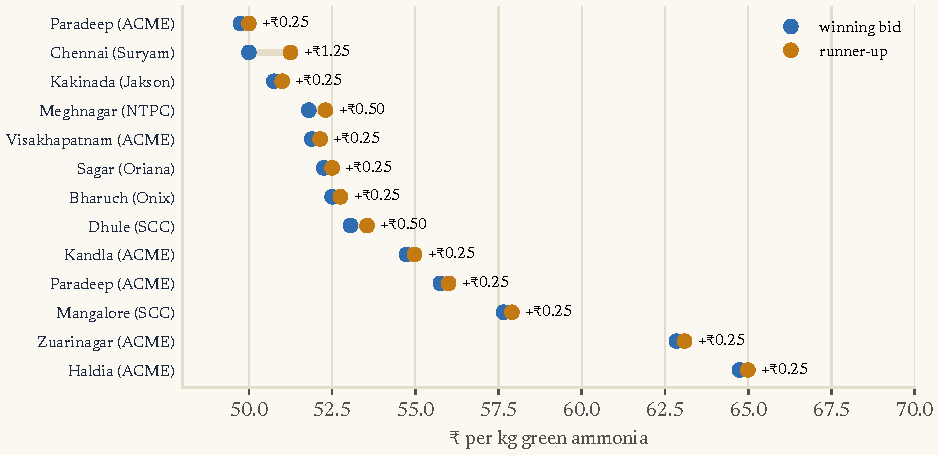
\includegraphics[width=\textwidth]{auction_gap.pdf}
\caption{Winning bid and runner-up in each of the 13 auctions. Data: \cite{seci2025}; \texttt{data/raw/seci\_mode2a\_tranche1\_bids.csv}.}
\end{figure}

\textbf{H1, bid structure.} In ten of thirteen auctions, the runner-up was exactly ₹0.25 behind the winner; the median gap is ₹0.25. ACME won 51\% of the volume. The money ``left on the table'' between winner and runner-up totals only about ₹22 crore a year. \emph{But we must be careful}: in an e-reverse auction, a uniform ₹0.25 gap is most likely the minimum bid decrement, so it tells us bidding was fierce at the end, not that costs were similar. We will therefore lean on H2 and H3, and test H1 against the auction rules once we have the bid logs. \confM

\begin{figure}[H]
\centering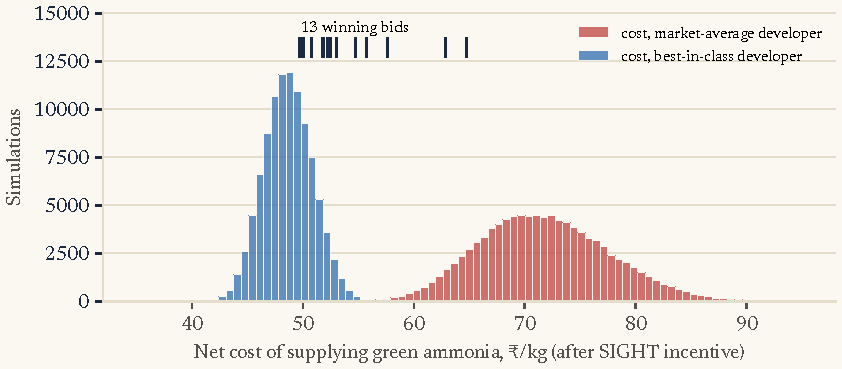
\includegraphics[width=\textwidth]{auction_cost.pdf}
\caption{Simulated net cost of green ammonia (100,000 draws each) against the 13 winning bids. Source: \texttt{auctions.py}.}
\end{figure}

\textbf{H2, cost coverage.} For a market-average alkaline developer, the median net cost is \textbf{₹71.5/kg}; the chance that a winning bid covers it is \textbf{0.5\%} (volume-weighted). For a best-in-class developer (cheap stacks, cheap power, long-life stacks, low-cost capital), the median falls to \textbf{₹48.6/kg} and the coverage rises to \textbf{91\%}. The auctions are not impossible; they are \emph{only} possible for the best. \confM

\begin{figure}[H]
\centering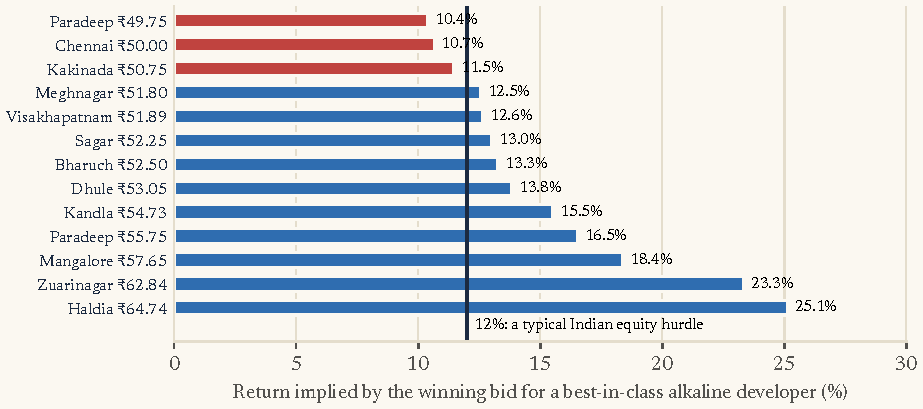
\includegraphics[width=\textwidth]{implied_wacc.pdf}
\caption{Return implied by each winning bid for a best-in-class developer. Source: \texttt{auctions.implied\_wacc}.}
\end{figure}

\textbf{H3, implied return.} Even for a best-in-class developer, the implied return ranges from \textbf{10.4\%} (IFFCO Paradeep, ₹49.75) to \textbf{25.1\%} (Haldia, ₹64.74), with a volume-weighted average of 14.0\%. Three awards (Paradeep IFFCO, Chennai and Kakinada) sit below a typical 12\% equity hurdle. Those are where delivery risk is concentrated. \confM

\begin{center}\tablefont
\begin{tabularx}{\textwidth}{@{}l L r r r c c c@{}}
\toprule
\thead{No.} & \thead{Buyer, location (winner)} & \thead{t/yr} & \thead{Win ₹} & \thead{Gap ₹} & \thead{Covers: avg} & \thead{best} & \thead{Implied}\\ \midrule
I & IFFCO, Kandla (ACME) & 100,000 & 54.73 & 0.25 & 0.0\% & 99.7\% & 15.5\%\\
II & IFFCO, Paradeep (ACME) & 100,000 & 49.75 & 0.25 & 0.0\% & 68.9\% & \textbf{10.4\%}\\
III & Madras Fertilizers, Chennai (Suryam) & 4,000 & 50.00 & 1.25 & 0.0\% & 72.5\% & \textbf{10.7\%}\\
IV & GNFC, Bharuch (Onix) & 50,000 & 52.50 & 0.25 & 0.0\% & 95.5\% & 13.3\%\\
V & Paradeep Phosphates, Paradeep (ACME) & 75,000 & 55.75 & 0.25 & 0.0\% & 100\% & 16.5\%\\
VI & Paradeep Phosphates, Zuarinagar (ACME) & 25,000 & 62.84 & 0.25 & 5.2\% & 100\% & 23.3\%\\
VII & Indorama, Haldia (ACME) & 20,000 & 64.74 & 0.25 & 11.0\% & 100\% & 25.1\%\\
VIII & MCF, Mangalore (SCC) & 15,000 & 57.65 & 0.25 & 0.2\% & 100\% & 18.4\%\\
IX & Coromandel, Visakhapatnam (ACME) & 50,000 & 51.89 & 0.25 & 0.0\% & 92.3\% & 12.6\%\\
X & Coromandel, Kakinada (Jakson) & 85,000 & 50.75 & 0.25 & 0.0\% & 82.3\% & \textbf{11.5\%}\\
XI & Krishna Phoschem, Meghnagar (NTPC REL) & 70,000 & 51.80 & 0.50 & 0.0\% & 91.7\% & 12.5\%\\
XII & Madhya Bharat Agro, Sagar (Oriana) & 60,000 & 52.25 & 0.25 & 0.0\% & 94.4\% & 13.0\%\\
XIII & Madhya Bharat Agro, Dhule (SCC) & 70,000 & 53.05 & 0.50 & 0.0\% & 97.4\% & 13.8\%\\
\bottomrule
\end{tabularx}
\end{center}

\begin{finding}[What the first results mean]
India's ammonia auctions have created a market in which \textbf{only a best-in-class developer can win and still earn its cost of capital, and a few awards look thin even for them}. That is not proof of a winner's curse; it is the condition under which one would appear. The test that would settle it is time: which awards reach financial close and commissioning on schedule. We will track all thirteen. \confM
\end{finding}

\subsection{Where the paper sits in the literature}
We checked every study in the Gemini literature review before relying on it \cite{gemlit2026}. Five survive as our core; two were mis-cited; several came from venues we will not cite.

\begin{center}\tablefont
\begin{xltabular}{\textwidth}{@{}P{34mm} L L@{}}
\toprule
\thead{Study} & \thead{What it does} & \thead{How we use it, or what we corrected}\\ \midrule
\endhead
Glenk \& Reichelstein (2019) \cite{glenk2019} & Shows when renewable hydrogen reaches cost parity, and how flexibility to sell power raises value. & Missing from the review; our anchor for LCOH logic.\\
Benalcazar \& Komorowska (2022) \cite{benalcazar2022} & Monte Carlo LCOH for Poland; power price and load factor dominate. & Validates our Monte Carlo approach.\\
Srettiwat et al.\ (2023) \cite{srettiwat2023} & Techno-economics of solar hydrogen for Belgium. & The review credited this to ``Al-Ghussain''; the authors are Srettiwat, Safari, Olcay and Malina (UHasselt).\\
Fabianek, Glensk \& Madlener (2024) \cite{fabianek2024} & Sequential real options for power-to-hydrogen, Germany and California. & Template for our expansion option.\\
Trivella (2025) \cite{trivella2025} & Electrolyser investment under market and technology uncertainty. & Supports staged investment and the AEM switch.\\
Kroniger \& Madlener (2014) \cite{kroniger2014} & Hydrogen storage as a real option for wind parks. & Early proof that flexibility has option value.\\
Zeyen, Victoria \& Brown (2023) \cite{zeyen2023} & Endogenous learning for electrolysers in a European model. & The review mis-attributed this; used for learning-rate ranges.\\
RMI (2025) \cite{rmi2025} & India production pathways: stand-alone on-site at \usd{}4.4--4.8/kg. & The review dated it 2024; it was published in July 2025.\\
Capen et al.\ (1971); Thaler (1988) \cite{capen1971,thaler1988} & The winner's curse in high-risk bidding. & Theoretical core of the paper.\\
\bottomrule
\end{xltabular}
\end{center}

\noindent The review also proposed a ``mean-reverting geometric Brownian motion'' for prices. Geometric Brownian motion does not mean-revert; the correct tool is the Schwartz one-factor model, a mean-reverting process on log prices \cite{schwartz1997}, which our \texttt{prices.py} implements and tests.

\subsection{What remains before submission}
\begin{itemize}
\item \textbf{Data.} The bid logs (if SECI releases them) to test H1 properly; real hourly solar and wind for each auction site; grey-ammonia import prices to fit the price model.
\item \textbf{Robustness.} Re-run H2 and H3 with each site's own resource profile, with Chinese stack prices, and with the developer's possible captive power.
\item \textbf{Extension.} Value each award's embedded option to walk away (the bid bond is the strike) to estimate the probability of non-delivery.
\item \textbf{Target journals.} \emph{Energy Policy} first (the policy question is central); \emph{Energy Economics} if the auction-theory part grows.
\end{itemize}
\newpage
